\chapter{研究方法}
\label{章:研究方法}

\section{拄好長度斷詞}
\label{節:拄好長度斷詞}

\begin{table}
\caption{長詞優先毋著的情形}
\label{表:長詞優先佇一寡例有問題}
\centering
\begin{tabular}{c|c}
方法 & 結果\\
\hline
長詞優先(對頭前) & 猶 掠做 唱歌 仔 戲 真 簡單\\
答案 & 猶 掠做 唱 歌仔戲 真簡單\\
\hline
長詞優先(對後壁) & 甚至 和 國 小學生 嘛 想 袂 開\\
答案 & 甚至 和 國小 學生 嘛 想 袂 開\\
\end{tabular}
\end{table}

\ref{節:閩南語斷詞}節講愛比較斷詞的方法,
定用的斷詞方法有\ref{節:長詞優先斷詞}節的長詞優先,
佇遮本論文提出一个「拄好長度斷詞」的方法。

%ㄍㄛˊ

因為長詞優先有時陣會揀著無好的組合,
親像表\ref{表:長詞優先佇一寡例有問題}內底的例,
長詞優先有的情形會斷毋著。
觀察這个情形,
第一組例是斷詞結果的詞數比答案閣加一个,
斷出來的詞傷濟矣。
第二組例是斷詞結果佮答案攏是斷詞兩个詞,
因為斷詞結果共四字攏分配做一字詞佮三字詞,
字數分配無齊勻。

綜合這兩个觀察,
本論文提出「拄好長度斷詞」。
成本函式親像公式\ref{式:拄好長度斷詞成本函式}是訂做一字詞1分、兩字詞1/2分、三字詞1/3分、四字詞1/4分、…,
斷詞的方法是演算法\ref{方法:拄好長度斷詞方法}配合維特比(Viterbi)算法揣出成本上低的斷詞法。
用面頂表的例,
算出來的成本會當看表\ref{表:拄好長度成本}

而且愛注意拄好長度斷詞毋是全部的語料攏會比長詞優先斷詞好,
親像表\ref{表:長詞優先比拄好長度斷詞較好的狀況}的例,
雖然拄好長度的總詞數比長詞優先閣較少,
毋過佮答案相比,
這个例猶原是長詞優先閣較好淡薄仔。

\begin{equation}
\label{式:拄好長度斷詞成本函式}
成本函式(n) = \frac{1}{n}
\end{equation}

\begin{algorithm}
  \caption{拄好長度斷詞}
  \label{方法:拄好長度斷詞方法}
  \begin{algorithmic}
    \REQUIRE 需要斷詞字數m, 辭典上長的詞字數k, 無斷詞的語句$[j_{1}, j_{2}, ... , j_{m}]$
    \ENSURE 斷詞成本, 斷詞的語句 %$[s_{1}, s_{2}, ... , s_{n}]$
%    \STATE \( 決定辭典上長的詞字數$k$ \)
%    \STATE 拄好長度斷詞(需要斷詞字數m,辭典上長的詞字數k)
		\IF{$n == 0$}
			\STATE \( 回傳 (0,\emptyset) \)
		\ENDIF
	    \STATE \(i\gets \argmin\limits_i \{\frac{1}{m-i}+(拄好長度斷詞(i,k)的成本) \} \),其中\(j_{i+1}, j_{i+2}, ... , j_{m}\)是辭典的一个詞,而且\(0 \leq m − k \leq i \leq m − 1\)
		\STATE 頂一層成本c,頂一層斷詞的語句S
	    \STATE \(成本c' \gets 頂一層成本c+\frac{1}{m-i}\)
	    \STATE \(斷詞的語句S' \gets 頂一層斷詞的語句S 加入詞 (j_{i+1}, j_{i+2}, ... , j_{m}) \)
		\STATE 回傳 (c',S')
%    \EndFunction
%    \STATE \( 拄好長度斷詞(m,k) \)
  \end{algorithmic}
\end{algorithm}

\begin{table}
\caption{拄好長度成本}
\label{表:拄好長度成本}
\centering
\begin{tabular}{c|c}
斷詞結果 & 拄好長度成本\\
\hline
猶 掠做 唱歌 仔 戲 真 簡單 & $…+\frac{1}{2}+\frac{1}{1}+\frac{1}{1}+…$\\
猶 掠做 唱 歌仔戲 真 簡單 & $…+\frac{1}{1}+\frac{1}{3}+…$\\
\hline
甚至 和 國 小學生 嘛 想 袂 開 & $…+\frac{1}{1}+\frac{1}{3}+…$\\
甚至 和 國小 學生 嘛 想 袂 開 & $…+\frac{1}{2}+\frac{1}{2}+…$\\
\end{tabular}
\end{table}

\begin{table}
\caption{長詞優先比拄好長度斷詞較好的狀況}
\label{表:長詞優先比拄好長度斷詞較好的狀況}
\centering
\begin{tabular}{c|l}
答案 & 七月半 鴨仔 毋 知 死活 \\
\hline
拄好長度 & 七 月半 鴨仔 毋知死 活 \\
長詞優先 & 七 月半 鴨仔 毋 知 死活 \\
\end{tabular}
\end{table}

\section{未知詞另外翻譯}
\label{節:未知詞另外翻譯}

\begin{figure}
\centerline{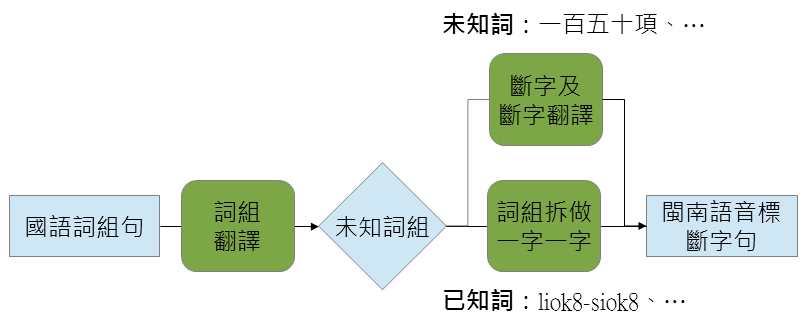
\includegraphics[keepaspectratio,width=40em]{圖/未知詞另外翻譯}}
\caption{未知詞另外翻譯流程}
\label{未知詞另外翻譯}
\end{figure}

對\ref{節:未知詞問題}節來看,
用斷詞翻譯會拄著未知詞的問題。
佇遮阮提出一个演算法\ref{方法:未知詞另外翻譯方法},
準若阮用斷詞翻譯模型,
拄著未知詞的時陣,
這个未知詞會使提予斷字翻譯模型去翻譯。

可比講「陸續 開放 一百五十項 的 規費」提予斷詞組模型翻譯,
得著「liok8-siok8 khai1-hong3 一百五十項 e5 規費」,
閣來共「一百五十項」佮「規費」這兩个詞組切做斷字「一 百 五 十 項」佮「規 費」,
閣擲去斷字模型翻譯,流程會當看圖\ref{未知詞另外翻譯}。

\begin{algorithm}
  \caption{未知詞另外翻譯}
  \label{方法:未知詞另外翻譯方法}
  \begin{algorithmic}
    \REQUIRE \( 原本華語句H = [h_{1}, h_{2},...] \)
    \ENSURE \( 翻譯閩南語句M = [m_{1}, m_{2},...m_{n}] \)
    \STATE \( M = [m_{1}, m_{2},...m_{n}] \gets 斷詞翻譯H的結果 \)
    
	\WHILE{存在$B = [m_{i} , m_{i+1} ,...m_{j}] 攏是未知詞,m_{i−1}, m_{j+1}是已知詞$}
		\STATE \( T \gets B提去斷字翻譯 \)
		\STATE 共M內的B換做T
	\ENDWHILE
  \end{algorithmic}
\end{algorithm}


\section{漢羅全羅對齊}
\label{節:漢羅全羅對齊}
佇\ref{節:臺文典藏}節有講著,
臺文典藏是提供漢羅佮全羅的對照,
因為阮的翻譯需要一个漢字對一个音標的一對一,
所以愛共臺文典藏伊原本一段對齊一段的語料改做一字對一字。
而且愛注意臺文典藏佇2006年完成,
教育部的漢字規範佇2007年才公佈,
所以\ji{⿰因}兩个的用字規範是無完全仝款的。
毋過臺文典藏的語料倩人整理的時陣內部有訂標準,伊的漢字有一半以上攏是會用得的。
本論文用字以教育部的為主,
對齊的做法是共漢羅逐字攏去對看覓全羅,
看漢羅字一字佮全羅一字的對應有佇字典內底無,
揣出上長的對應組合。

%有1個少年人;伊抵tng7 teh 想
%U7 chit8 e5 siau3-lian5 lang5; i tu2-tng7 teh siuN7 phok-su7 lun7-bun5, 

\section{補全漢佮全羅}
\label{節:補全漢佮全羅}
佇\ref{節:整理語料}節有講著,
閩南語語料的完整資訊有全漢、全羅、斷詞三項,
若全部的語料攏有這三種資訊,
翻譯效果會閣較好。

斷詞的部份佇\ref{節:拄好長度斷詞}節有討論矣,
這節的重點是下佇按怎自動整理語料,
予\ji{⿰因}有完整的全漢佮全羅資訊,
也就是替\ji{⿰因}補起哩欠的漢字佮羅馬音標。

因為有的詞可能一字音標、一字是漢字,
親像「彰化」,寫做「tsiong-化」。
本論文提出一个做法,
整理語料的時猶原用斷詞方法,
毋過用的辭典愛小可仔改變,
逐个詞的全部形式攏愛加佇辭典內底,
閣愛加
「\tsoo{彰}{}{}\tsoo{化}{}{}」、
「\tsoo{彰}{}{}\tsoo{huà}{}{}」、
「\tsoo{彰}{}{}\tsoo{化}{⿳⿳⿳ㄏㄨㄚ˪}{huà}」、
「\tsoo{tsiong}{}{}\tsoo{化}{}{}」、
「\tsoo{tsiong}{}{}\tsoo{huà}{}{huà}」、
「\tsoo{tsiong}{}{}\tsoo{化}{}{}」、
「\tsoo{彰}{⿳⿳ㄐㄧㆲ}{tsiong}\tsoo{化}{}{}」、
「\tsoo{彰}{⿳⿳ㄐㄧㆲ}{tsiong}\tsoo{huà}{}{}」、
「\tsoo{彰}{⿳⿳ㄐㄧㆲ}{tsiong}\tsoo{化}{⿳⿳⿳ㄏㄨㄚ˪}{huà}」
%「\tsoo{彰}{}{}\tsoo{化}{}{}」、
%「\tsoo{彰}{}{}\tsoo{}{⿳⿳⿳ㄏㄨㄚ˪}{huà}」、
%「\tsoo{彰}{}{}\tsoo{化}{⿳⿳⿳ㄏㄨㄚ˪}{huà}」、
%「\tsoo{}{⿳⿳ㄐㄧㆲ}{tsiong}\tsoo{化}{}{}」、
%「\tsoo{}{⿳⿳ㄐㄧㆲ}{tsiong}\tsoo{}{⿳⿳⿳ㄏㄨㄚ˪}{huà}」、
%「\tsoo{}{⿳⿳ㄐㄧㆲ}{tsiong}\tsoo{化}{⿳⿳⿳ㄏㄨㄚ˪}{huà}」、
%「\tsoo{彰}{⿳⿳ㄐㄧㆲ}{tsiong}\tsoo{化}{}{}」、
%「\tsoo{彰}{⿳⿳ㄐㄧㆲ}{tsiong}\tsoo{}{⿳⿳⿳ㄏㄨㄚ˪}{huà}」、
%「\tsoo{彰}{⿳⿳ㄐㄧㆲ}{tsiong}\tsoo{化}{⿳⿳⿳ㄏㄨㄚ˪}{huà}」
攏總九種\footnote{一个字的資訊可能是「漢字」、「音標」、「漢字音標攏有」三種其中一種。
兩字,攏總$3^{2}=9$種}。

%為著查字典的速度閣較緊,
%就親像圖XX仝款,
%逐个詞一字一字處理落來,
%逐字分做漢字、音標、一對一三个點,
%第二个字閣佇這三个點閣生落去,
%毋過第一个字有佮別的詞仝款,
%就會使公家一个點,
%親像「彰化」「將來」「將軍庄」,
%因為限制上長四字詞\footnote{照教育部的「臺灣閩南語羅馬字拼音方案連字符使用原則」,
%有可能有五字詞,毋過這擺實驗限制四字詞},
%一个詞上濟產生120點\footnote{第一層加到第四層,$3^{1}+3^{2}+3^{3}+3^{4}=120$},
%毋過揣候選詞的時間複雜度是$O(1)$。

決定斷詞斷佇佗位了後,
逐个斷詞的所在可能有超過一个的候選詞,
%「彰化的米誠好食」,
上尾閣用語言模型,
配合維特比算法,
揀出機率上懸的語句。


\section{語言分類特徵}
\label{節:語言分類特徵}

\ref{節:語言分類}節有講,
閩南語佮華語以字為單位的語言模型效果無好,
為著予電腦會當分別閩南語佮華語,
阮就愛準備幾項閩南語佮華語無仝的特徵。
本論文提出一个以斷詞資訊做判斷特徵的方法,
除了以斷詞算語言模型以外,
閣加入斷詞了一字詞、兩字詞、三字詞、四字詞的詞數,
毋過按呢猶原無夠。

閩南語佮華語上大差別就是用詞無仝,
閩南語寫「食飯」、「無法度」,
華語寫「吃飯」、「沒辦法」,
所以阮揀定用詞出來,
當作阮的特徵之一。

毋過閩南語佮華語有誠濟共同詞,
親像「火車」、「電腦」,
\ji{⿰因}寫法是仝款的,
阮袂使直接提定用詞來做,
因為內底會有共同詞,
所以阮愛揀出無共同詞的「特徵詞」。

選特徵詞的方法是先統計閩南語語料佮華語語料,
分別揣出n个定用詞\footnote{有算標點符號},
了後揀出頭前m个閩南語定用詞,
而且這m个閩南語定用詞無出現佇華語n个定用詞,
這m个詞阮就號做閩南語特徵詞。
華語部份嘛仝款,
揀出頭前m个華語定用詞,
這m个詞無出現佇閩南語的n个定用詞,
這m个詞就是華語的特徵詞。

佇遮阮設$定用詞數量是n=7000,特徵詞數量是m=3000$來揣華語閩南語的特徵詞,
頭幾个定用詞佮特徵詞佇表\ref{表:定用詞佮特徵詞},
「\tsoo{的}{⿳ㆤˊ}{ê}」佮「\tsoo{伊}{⿳ㄧ }{i}」攏是閩南語的定用詞,
毋過這兩个詞「\tsoo{的}{⿳⿳˙ㄉㄜ}{}」佮「\tsoo{伊}{⿳ㄧ }{}」華語攏會用著,
所以袂使做閩南語的特徵詞。
親像「\tsoo{佇}{⿳⿳ㄉㄧ˫}{tī}」華語就罕得用著「\tsoo{佇}{⿳⿳ㄓㄨˋ}{}」,
就會使當做閩南語的特徵詞。

有斷詞、語言模型佮特徵詞的資訊,
就會當親像圖\ref{圖:判斷語言架構}仝款,
交予分類器做語言分類。

\begin{table}
\caption{n=7000、m=3000的頭前九个定用詞佮特徵詞}
\label{表:定用詞佮特徵詞}
\centering
\begin{tabular}{c|cccccccccc}
第幾个 & 1 & 2 & 3 & 4 & 5 & 6 & 7 & 8 & 9\\
\hline
閩南語定用詞 &
\tsoo{的}{⿳ㆤˊ}{ê} & \tsoo{伊}{⿳ㄧ }{i} & \tsoo{有}{⿳ㄨ˫}{ū} &
\tsoo{是}{⿳⿳ㄒㄧ˫}{sī} & \tsoo{我}{⿳⿳⿳ㆣㄨㄚˋ}{guá} & \tsoo{人}{⿳⿳ㄌㄤˊ}{lâng} &
\tsoo{無}{⿳⿳ㆠㄜˊ}{bô} & \tsoo{講}{⿳⿳ㄍㆲˋ}{kóng} & \tsoo{佇}{⿳⿳ㄉㄧ˫}{tī} & …\\
\hline
華語定用詞 &
\tsoo{的}{⿳⿳˙ㄉㄜ}{} & \tsoo{是}{⿳ㄕˋ}{} & \tsoo{在}{⿳⿳ㄗㄞˋ}{} &
\tsoo{一}{⿳ㄧ }{} & \tsoo{有}{⿳⿳ㄧㄡˇ}{} & \tsoo{了}{⿳⿳˙ㄌㄜ}{} &
\tsoo{不}{⿳⿳ㄅㄨˋ}{} & \tsoo{我}{⿳⿳ㄨㄛˇ}{} & \tsoo{個}{⿳⿳˙ㄍㄜ}{} & …\\
\hline
閩南語特徵詞 &
\tsoo{佇}{⿳⿳ㄉㄧ˫}{tī} & \tsoo{个}{⿳ㆤˊ}{ê} & \tsoo{閣}{⿳⿳ㄍㄜㆷ}{koh} &
\tsoo{攏}{⿳⿳ㄌㆲˋ}{lóng} & \tsoo{佮}{⿳⿳ㄍㄚㆴ}{kap} & \tsoo{\ji{⿰因}}{⿳ㄧㄣ}{in} &
\tsoo{咧}{⿳⿳ㄉㆤㆷ}{teh} & \tsoo{咱}{⿳⿳ㄌㄢˋ}{lán} & \tsoo{彼}{⿳⿳ㄏㄧㆵ}{hit} & …\\
\hline
華語特徵詞 &
\tsoo{我}{⿳⿳ㄨㄛˇ}{}\tsoo{們}{⿳⿳˙ㄇㄣ}{} & \tsoo{很}{⿳⿳ㄏㄣˇ}{} & \tsoo{她}{⿳ㄊㄚ}{} &
\tsoo{沒}{⿳⿳ㄇㄟˊ}{}\tsoo{有}{⿳⿳ㄧㄡˇ}{} & \tsoo{或}{⿳⿳⿳ㄏㄨㄛˋ}{} & \tsoo{他}{⿳ㄊㄚ}{}\tsoo{們}{⿳⿳˙ㄇㄣ}{} &
\tsoo{更}{⿳⿳ㄍㄥˋ}{} & \tsoo{則}{⿳⿳ㄗㄜˊ}{} & \tsoo{把}{⿳⿳ㄅㄚˇ}{} & …\\
\end{tabular}
\end{table}

\begin{figure}
\centerline{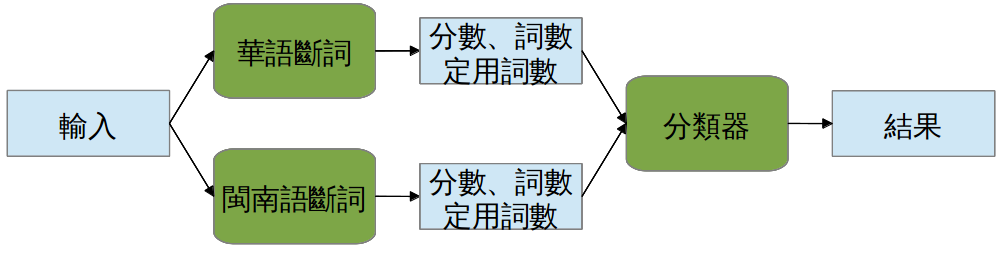
\includegraphics[keepaspectratio,width=40em]{圖/判斷語言架構}}
\caption{判斷語言流程}
\label{圖:判斷語言架構}
\end{figure}
